\documentclass[a4paper]{article}
\usepackage{graphicx}
\usepackage[a4paper, left=5mm, right=5mm, top=5mm, bottom=5mm]{geometry}
%\geometry{paperwidth=210mm, paperheight=2000pt, left=5pt, top=5pt}
\usepackage[utf8]{inputenc}
\usepackage[english,russian]{babel}
\usepackage{indentfirst}
\usepackage{tikz} %Рисование автоматов
\usetikzlibrary{automata,positioning,arrows,trees,calc}
\usepackage{amsmath}
\usepackage[makeroom]{cancel} % зачеркивание
\usepackage{multicol,multirow} %Несколько колонок
\usepackage{hyperref}
\usepackage{tabularx}
\usepackage{amsfonts}
\usepackage{wrapfig}
\usepackage{amssymb}
\DeclareMathOperator*{\argmin}{arg\,min}
\usepackage{listings}
\usepackage{wasysym}
\date{2014.12.25}
\author{Сергей~Володин, 274 гр.}
\newcommand{\matrixl}{\left|\left|}
\newcommand{\matrixr}{\right|\right|}
% названия автоматов  (rubtsov)
\def\A{{\cal A}}
\def\B{{\cal B}}
\def\C{{\cal C}}

\title{Эффект Эйнштейна --- де Хааза\\(реферат)}

%+= и -=, иначе разъезжаются...
\newcommand{\peq}{\mathrel{+}=}
\newcommand{\meq}{\mathrel{-}=}
\newcommand{\deq}{\mathrel{:}=}
\newcommand{\plpl}{\mathrel{+}+}

% пустое слово  (rubtsov)
\def\eps{\varepsilon}

\def\eqdef{\overset{\mbox{\tiny def}}{=}}
\newcommand{\niton}{\not\owns}


\newcommand{\smalll}[1]{\overline{\overline{#1}}}
\newcommand{\smallo}{\bar{\bar{o}}}
\begin{document}
\maketitle
\section*{Введение}
В 1820 году Эрстед выяснил, что магнитное поле может быть создано не только постоянными магнитами, но еще и токами. Получалось, что источников магнитного поля может быть два типа: токи и постоянные магниты. В попытке разобраться в этой ситуации и выяснить природу магнетизма, сведя два типа к одному, Ампер выдвинул гипотезу, согласно которой в постоянных магнитах циркулируют без сопротивления молекулярные токи, которые и создают магнитное поле. В 1915 году Эйнштейн и де Хааз провели эксперимент, который должен был подтвердить гипотезу Ампера.

\section*{Классическое обоснование (модель Бора, орбитальный момент)}
В модели атома Бора (1913) электрон вращается по круговой орбите. Из-за этого, во-первых, он имеет момент импульса, во-вторых, магнитный момент, так как электрон~--- заряженная частица. Поэтому следует ожидать, что изменение магнитных свойств (намагничивание) будет приводить к изменению механических: тело начнет вращаться. Такой эффект и наблюдали Эйнштейн и де Хааз.

Рассмотрим атом модели Бора. Электрон с зарядом $e=-1.6\cdot 10^{-19}$ Кл движется вокруг ядра с зарядом $Z|e|$. Момент импульса электрона $L=mvr=m\frac{2\pi r}{T}r=m 2\pi r^2 \nu,$ где $\nu$~--- частота обращения электрона вокруг ядра. Магнитный момент $M=IS=e\nu\pi r^2$. Отсюда получаем гиромагнитное отношение $\gamma\eqdef \frac{M}{L}=\frac{e\nu\pi r^2}{2m\pi\nu r^2}=\frac{e}{2m}\approx -8.79\cdot 10^{10}\frac{\mbox{Кл}}{\mbox{кг}}$. Обратная величина $\frac{1}{\gamma}=-1.14\cdot 10^{-11}\frac{\mbox{кг}}{\mbox{Кл}}$.

В векторном виде гиромагнитное соотношение записывается как $\vec{M}=\gamma\vec{L}$

Из-за наличия такого соотношения изменение намагниченности образца приведет к его вращению как целого. Действительно, пусть $\vec{L}_1$~--- сумма всех орбитальных моментов импульса электронов, $\vec{L}_2$~--- момент импульса тела как целого. Полный момент сохраняется: $0=\frac{d}{dt}(\vec{L}_1+\vec{L}_2)$, откуда $\frac{d\vec{L}_2}{dt}=-\frac{d\vec{L}_1}{dt}=-\frac{1}{\gamma}\frac{d}{dt}\sum\limits_i \vec{M}_i$, где $\vec{M}_i$~--- орбитальные магнитные моменты всех атомов. Это можно интерпретировать так: на тело как целое действует момент силы $\vec{\tau}=-\frac{1}{\gamma}\frac{d}{dt}\vec{M}_\Sigma$., то есть, тело начнет вращаться.

Пусть внешнее магнитное поле изменяется с $\vec{B}_0$ до противоположного $-\vec{B}_0$. Пусть $B_0$ достаточно сильное, т.е. намагниченность достигает насыщения и изменяется с $\vec{I}s$ на противоположное $-\vec{I}_s$. Изменение момента импульса $J\Delta \omega=\int\limits_0^t\tau dt=\int\limits_0^t -\frac{1}{\gamma}\frac{d}{dt}(M_\Sigma) dt=-\frac{\Delta M_\Sigma}{\gamma}$. Тогда $\Delta\omega=-\frac{4I_s}{\gamma\rho R^2}\approx 0.6\cdot 10^{-8}\mbox{с}^{-1}$, если взять $J=\frac{1}{2}MR^2$, $R=10^{-3}\mbox{м}$, $I_s=1\mbox{Тл}$, $\rho=7800\frac{\mbox{кг}}{\mbox{м}^3}$.
\newpage
\section*{Эксперимент}
\begin{center}
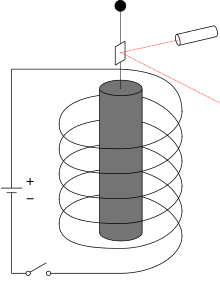
\includegraphics[width=5cm]{lab.png}
\end{center}
Рассмотрим подвешенный на нити цилиндр, помещенный в катушку с током $i$, которая создает магнитное поле. Запишем уравнение вращательных колебаний ($\beta,\omega_0$~--- параметры собственных колебаний):
$$\ddot{\alpha}+2\beta\dot{\alpha}+\omega_0^2\alpha=\frac{1}{J}\tau$$
Пропустим через катушку синусоидальный ток частоты $\omega$: $i=A\sin\omega t$. Момент сил $\tau$ в таком случае не обязан быть синусоидальным, так как кривая намагничивания нелинейна (петля гистерезиса) при достаточно больших внешних полях, а именно такие поля и были использованы.
\begin{center}
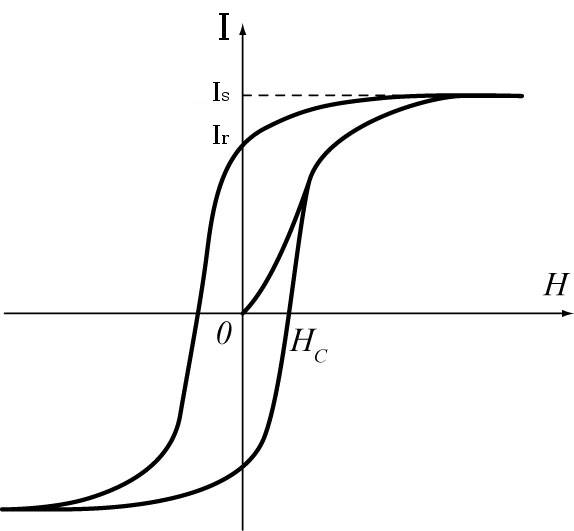
\includegraphics[width=5cm]{hyst.png}
\end{center}
Эйнштейном и де Хаазом был получен график зависимости тока от времени и момента сил от времени. Ток синусоидальный, а момент сил (вторая кривая)~--- нет.
\begin{center}
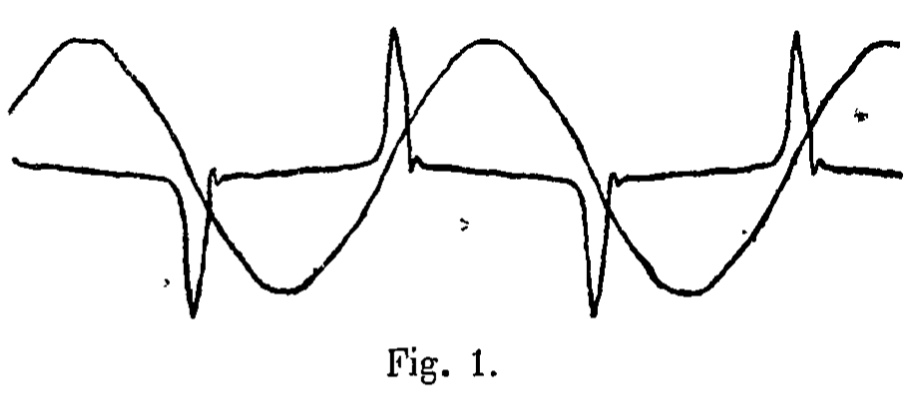
\includegraphics[width=10cm]{fig1.png}
\end{center}
<<Пик>> возникает при смене знака тока, что соответствует смене знака внешнего магнитного поля, т.е. движению вдоль кривой гистерезиса вблизи нуля, где производная $\frac{dI}{dt}$ как раз велика. <<Плоские>> участки соответствую движению по асимптотам (насыщение).

Разложим момент сил в ряд Фурье на периоде $T=\frac{2\pi}{\omega}$ как четную функцию: $\tau=\sum\limits_{n=1}^{\infty}B_n\cos n\omega t$. В результирующих колебаниях амплитуда велика только для первого члена при $\omega\approx\omega_0$ (резонанс). Вычислим $B_1$. На отрезке $t\in[-\frac{\pi}{2\omega},\frac{3\pi}{2\omega}]$ наблюдается два пика, первый вверх, второй вниз. Проинтегрируем разложение для момента, умноженное на $\cos\omega t$ по указанному периоду (<<перекрестные>> члены уйдут): $$\int\limits_{-\frac{\pi}{2\omega}}^{\frac{3\pi}{2\omega}}\tau\cos\omega tdt=\int\limits_{-\frac{\pi}{2\omega}}^{\frac{3\pi}{2\omega}}B_1\cos^2\omega tdt=\frac{\pi}{\omega}B_1$$

В первом пике ($t\approx0$) значение $\cos\omega t\approx 1$, во втором пике ($t\approx \frac{\pi}{\omega}$) значение $\cos\omega t\approx -1$. Интеграл по каждому пику, как показано выше, равен $\int \tau dt=-\frac{1}{\gamma}\Delta M_\Sigma=-\frac{2}{\gamma}M_s$, где $M_s=I_sV$~--- суммарный магнитный момент при насыщении. В итоге интеграл слева можно оценить как $-\frac{4}{\gamma}I_sV$. Получаем соотношение $B_1=-\frac{4I_sV\omega}{\pi\gamma}$.

Найдем решение уравнения колебаний, оставив в правой части только член с $\cos\omega t$, который дает максимальную среди всех членов амплитуду колебаний (резонансный):
$$
\ddot{\alpha}+2\beta\dot{\alpha}+\omega_0^2\alpha=\frac{B_1}{J}\cos\omega t
$$
Собственные колебания не учитываем, так как они затухающие (ими можно пренебречь). Частное решение ищем в виде $\alpha(t)=\mbox{Re} Ae^{i\omega t}$, получаем $A=\frac{B_1/J}{(\omega_0^2-\omega^2)+2\beta i\omega}$, откуда $\alpha=\mbox{Re}(Ae^{i\omega t})=\mbox{Re}(A)\mbox{Re}(e^{i\omega t})-\mbox{Im}(A)\mbox{Im}(e^{i\omega t})=|A|\cos(\omega t-\varphi)$, $\begin{cases}
\cos\varphi=\frac{\mbox{Re}A}{|A|}\\
\sin\varphi=\frac{\mbox{Im}A}{|A|}\\
\end{cases}$

В опыте была получена зависимость амплитуды колебаний от частоты тока в катушке, $|A|(\omega)$~--- резонансная кривая, которая представлена графически. По оси ординат отложена величина, пропорциональная $|A|$: угол измерялся при помощи зеркальца, жестко закрепленного на торце цилиндра, луча света и шкалы на расстоянии $L=1.45\, \mbox{м}$, откуда $\Delta l=L\tan(2|A|)\approx2|A| L$ и $|A|=\frac{1}{2}\arctan\frac{\Delta l}{L}\approx\frac{\Delta l}{2L}$
\begin{center}
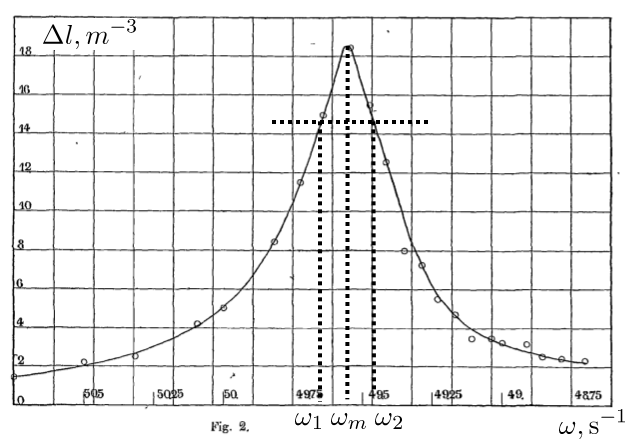
\includegraphics[width=15cm]{res}
\end{center}
Из полученной резонансной кривой найдем $\gamma$. Фиксируем значение $|A|$ и найдем две частоты $\omega_1$ и $\omega_2$ соответствующие этому $|A|$ на кривой. Рассмотрим также резонансную частоту $\omega_m\equiv\omega_0$. Обозначим в выражении для $|A|$ константу $\mu$, содержащую искомое $\gamma$:
$$
|A|(\omega)=\frac{|B_1|}{J}\left((\omega_0^2-\omega^2)^2+4\beta^2\omega^2\right)^{-1/2}=\underbrace{\frac{4I_sV}{\pi|\gamma|}}_{\mu}\left(\frac{(\omega_0^2-\omega^2)^2}{\omega^2}+4\beta^2\right)^{-1/2}
$$
Тогда $(\frac{\mu}{|A|})^2=\frac{(\omega_0^2-\omega^2)^2}{\omega^2}+4\beta^2$. В резонансе $(\omega=\omega_0\equiv\omega_m)$ найдем $\frac{\mu}{|A|_m}=2\beta$.

Для двух точек с совпадающими $|A|$ найдем $(\frac{\mu}{|A|_{1,2}})^2=\frac{(\omega_0^2-\omega_1^2)^2}{\omega_1^2}+4\beta^2=\frac{(\omega_0^2-\omega_2^2)^2}{\omega_2^2}+4\beta^2$. Приравняем второе и третье выражения, получим $\omega_0=\sqrt{\omega_1\omega_2}$.

Рассмотрим разницу $(\frac{\mu}{|A|_{1,2}})^2-(\frac{\mu}{|A|_m})^2\boxed{=}$, подставим туда найденные $\omega_0$ и $\frac{\mu}{|A|_m}$, получим $\boxed{=}(\omega_1-\omega_2)^2$.

Обозначим $b\eqdef\frac{|A|_{1,2}}{|A|_m}$~--- безразмерный параметр (отношение выбранной амплитуды к максимальной амплитуде) и $4\pi\nu=\omega_2-\omega_1$~--- половина разницы частот между $\omega_1$ и $\omega_2$.

Подставим обозначенные параметры в найденное соотношение: $(\frac{\mu}{|A|_m})^2(\frac{1}{b^2}-1)=(4\pi)^2\nu^2$. Выразим из него $\mu$ и приравняем с определением $\mu$:
$$
\frac{4I_sV}{\pi|\gamma|}\eqdef\mu=4\pi\nu|A|_m\sqrt{\frac{b^2}{1-b^2}}
$$
отсюда получим $\frac{1}{|\gamma|}=\frac{\pi^2\nu|A|_m}{I_sV}\sqrt{\frac{b^2}{1-b^2}}$

Таким образом, выбрав любую амплитуду $|A|_{1,2}$, мы можем рассчитать значение $\gamma$. Поэтому, если все предположения (например, линейность члена, отвечающего за затухание; отсутствие зависимости $\gamma$ от величины поля, ...) верны, величина $\nu\sqrt{\frac{b^2}{1-b^2}}$ не должна зависеть от выбора $|A|$. В проведенном Эйнштейном и де Хаазом опыте это утверждение верно при достаточно близких к максимальному $|A|_m$ значениях $|A|_{1,2}$, т.е., вблизи резонанса:
$$
\begin{array}{|c|c|}
\hline
\Delta l, 10^{-3}\mbox{м} & \nu\sqrt{\frac{b^2}{1-b^2}}, \mbox{с}^{-1}\\\hline
15 & 0.120 \\\hline
12 & 0.130 \\\hline
9  & 0.124 \\\hline
7  & 0.121 \\\hline
5  & 0.114 \\\hline
4  & 0.108 \\\hline
3  & 0.0957 \\\hline
\end{array}
$$

Найдем среднее значение величины $x\eqdef\nu\sqrt{\frac{b^2}{1-b^2}}$ по первым четырем значениям из таблицы, где величина остается постоянной: $x_{\mbox{ср.}}\approx 0.124 \mbox{с}^{-1}$.

Найдем остальные величины, входящие в выражение для $\frac{1}{|\gamma|}$.
%Измеряя амплитуду колебаний при различных частотах тока в катушке, можно построить резонансную кривую, из нее найдем величину константы $\gamma$ и сравним его с теоретическим ($\frac{2m}{e}$)
\section*{Источники погрешностей и их устранение}
\section*{Результаты и квантовая физика}
Эйнштейном и де Хаазом было получено экспериментально гиромагнитное отношение $\gamma=...$ с погрешностью $10 \%$. Тем не менее, в последующих работах ..., где был выполнен похожий эксперимент ..., соотношение получилось равным ... (в два раза больше). Это указывает на то, что магнетизм связан не только с орбитальным, а еще и со спиновым угловым моментом. То есть, хотя и эксперимент не подтверждает существование молекулярных токов Ампера, но косвенно подтверждает существование спина.
\begin{thebibliography}{}
\item В.Я.Френкель. УФН т.128, (1979) с.545.
\item A. Einstein, W. J. de Haas, Experimental proof of the existence of Ampère's molecular currents (in English), Koninklijke Akademie van Wetenschappen te Amsterdam, Proceedings, 18 I, pp. 696–711 (1915).
\end{thebibliography}
\end{document}